\documentclass{beamer}
\usepackage[utf8]{inputenc}
\usepackage{mathrsfs}
\usepackage{xcolor}
\usepackage[T1]{fontenc}
\usepackage[normalem]{ulem}
\usepackage{graphicx}

\setbeamercovered{invisible}
\setbeamercovered{%
  again covered={\opaqueness<1->{15}}}

\usetheme{Antibes}

\title{Gene expression clustering for single-cell RNA sequencing data}
\author{C. \textsc{Réda}\\supervised by G. \textsc{Ilsley} \& N. \textsc{Luscombe}} 
\institute{OIST, \textbf{Genomics and Regulatory Systems} Unit, Japan}
\date{March, $1^{st}$ - July, $31^{st}$}

\begin{document}
\maketitle
\tableofcontents
\setlength{\parindent}{1cm}

\addtobeamertemplate{footline}{\insertframenumber / \inserttotalframenumber}

\section{My internship}

\begin{frame}
\tableofcontents[currentsection]
\end{frame}

\subsection{Hosting institution \& research team}

\begin{frame}
\frametitle{My internship from March, $1^{st}$ to July, $31^{st}$}

\begin{center}

\begin{figure}
\centering
\subfigure\includegraphics[scale=0.2]{Images/okinawa.png}
\subfigure\includegraphics[scale=0.35]{Images/oist.jpg}
\caption{from \textbf{Google Maps \& OIST website}}
\end{figure}

\begin{flushcenter} Okinawa Institute of Science and Technology (OIST) \end{flushcenter}\\
\pause
\begin{flushcenter} \bf Genomics and Regulatory Systems (Luscombe Unit) \end{flushcenter}\\
\end{center}

\end{frame}

\subsection{Motivation}

\begin{frame}
\frametitle{Projects in the Luscombe Unit}

\begin{itemize}[<+>]
\item Study of \textit{Ciona intestinalis}. 
\item Culture of \textit{Oikopleura dioica}. 
\item Research on the fly and the yeast, etc.
\end{itemize}

\begin{figure}
\centering
\subfigure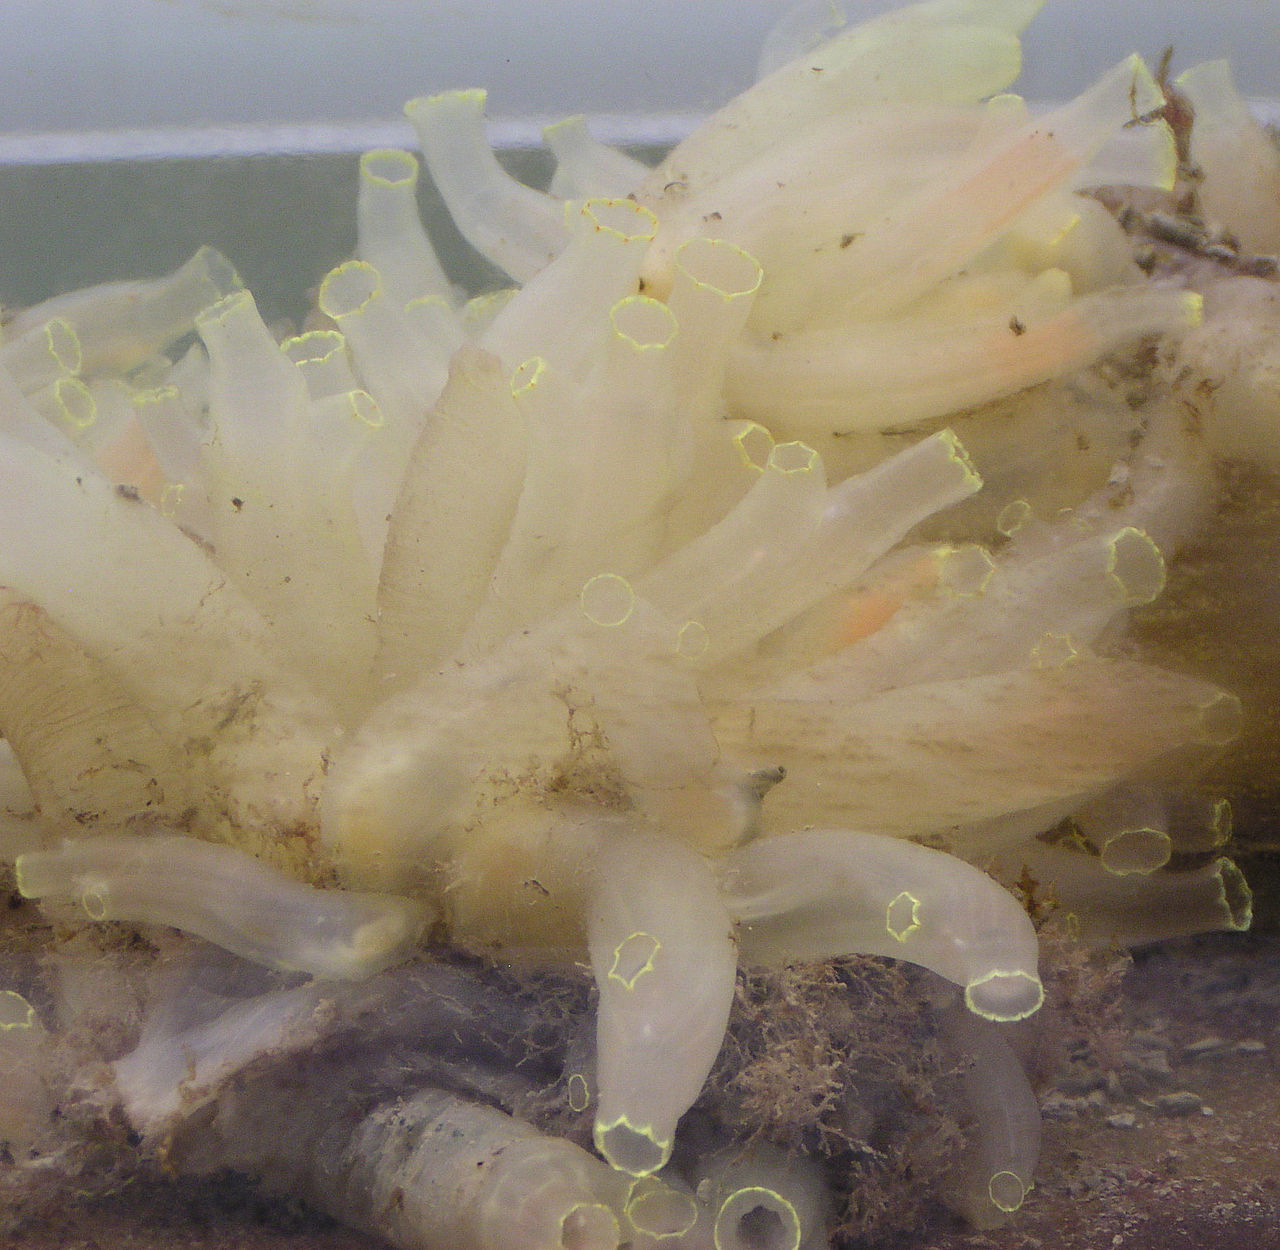
\includegraphics[scale=0.07]{Images/ciona.jpg}
\subfigure\includegraphics[scale=0.28]{Images/oiko.png}
\subfigure\includegraphics[scale=0.35]{Images/yeast.jpg}
\caption{Ciona \textbf{(Wikipédia)} \& Oikopleura \textbf{(OikoBase)} \& Yeast \textbf{(NPR)}}
\end{figure}

\end{frame}

\section{My work}

\begin{frame}
\tableofcontents[currentsection]
\end{frame}

\subsection{General context} 

\begin{frame}
\tableofcontents[currentsubsection]
\end{frame}

\begin{frame}
\frametitle{RiboNucleic Acid (RNA)}

\begin{block}{Definition}DNA-like molecule that allows \textbf{gene expression}, and helps \textbf{producing proteins}.\end{block}

\begin{figure}
\center
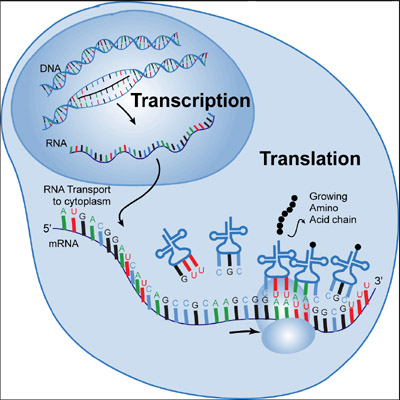
\includegraphics[scale=0.8]{Images/all.png}
\end{figure}

\end{frame}

\begin{frame}
\frametitle{RNA sequencing}

\begin{block}{Single-Cell RNA Sequencing (scRNAseq)}
\begin{center}
Gets the 4-letter (A, G, U, C) code that controls protein production in a given cell. 
\end{center}
\end{block}

\pause
\begin{block}{Gene expression level}
\begin{center}
In given sample and gene $g$, count of the \textbf{reads} which match with the coding sequence of $g$.
\end{center}
\end{block}

\end{frame}

\begin{frame}
\frametitle{Gene expression matrix}

\begin{block}{Gene expression matrix}
\begin{center}
For a given set of samples, matrix that contains the gene expression \textbf{profiles} (for all genes) for each sample $\thicksim$ cell. 
\end{center}
\end{block}

\begin{figure}
\centering
\includegraphics[scale=0.55]{Images/matrix.png}
\caption{From \textbf{[Tintori et al., 2016]}}
\end{figure}
 
\end{frame}

\begin{frame}
\frametitle{Main focus}

\begin{alertblock}{Gene expression pattern}
\begin{center}
Gene expression profile specific to a given \textbf{cell type} $\thicksim$ \textbf{cell functional family}. 
\end{center}
\end{alertblock}

\begin{center}
a given \textbf{gene expression pattern} on a set of \textbf{important genes}\\
$ \equiv $ 
a cell function
\end{center}

\end{frame}

\begin{frame}
\frametitle{Why are gene expression profiles studied?}

\begin{itemize}[<+>]
\item To find cell sub-populations in a tumor \textbf{[Patel et al., 2014]}.
\item To study of the developmental stages of an organism\\ \textbf{[Treutlein et al., 2014]}.
\item To discover new cell types \textbf{[Usoskin et al., 2015]}, etc.
\end{itemize}

\begin{figure}
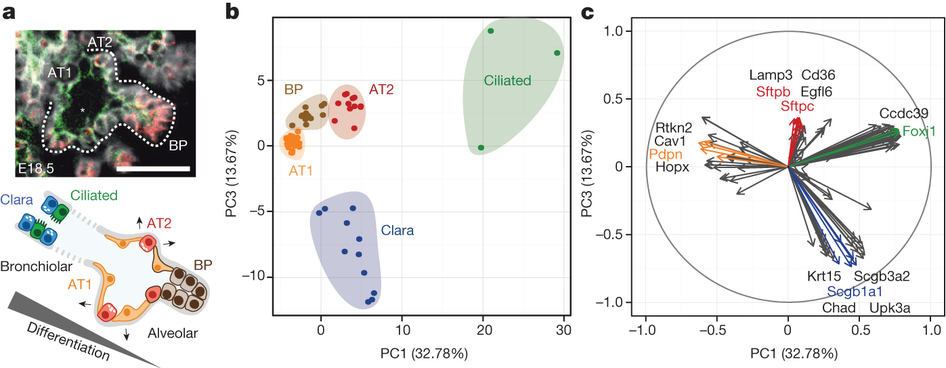
\includegraphics[scale=0.3]{Images/cellclustering.jpg}
\caption{Mouse cell \textbf{clustering} (grouping) from \textbf{[Treutlein et al., 2014]}}
\end{figure}

\end{frame}

\subsection{Objectives}

\begin{frame}
\tableofcontents[currentsubsection]
\end{frame}

\begin{frame}
\frametitle{Motivation}

\begin{alertblock}{My contributions}
\bigskip
\begin{enumerate}[<+>]
\item To design a visualization tool for \textbf{gene expression profiles}.
\item To perform a benchmark on different \textbf{cell clustering algorithms}.
\item To design a model for single-cell gene expression. 
\end{enumerate}
\bigskip
\end{alertblock}

\end{frame}

\section{My contribution}

\begin{frame}
\tableofcontents[currentsection]
\end{frame}

\subsection{Visualization of single-cell RNA sequencing data}

\begin{frame}
\tableofcontents[currentsubsection]
\end{frame}

\begin{frame}
\frametitle{Demonstration}

\begin{figure}
\centering
\subfigure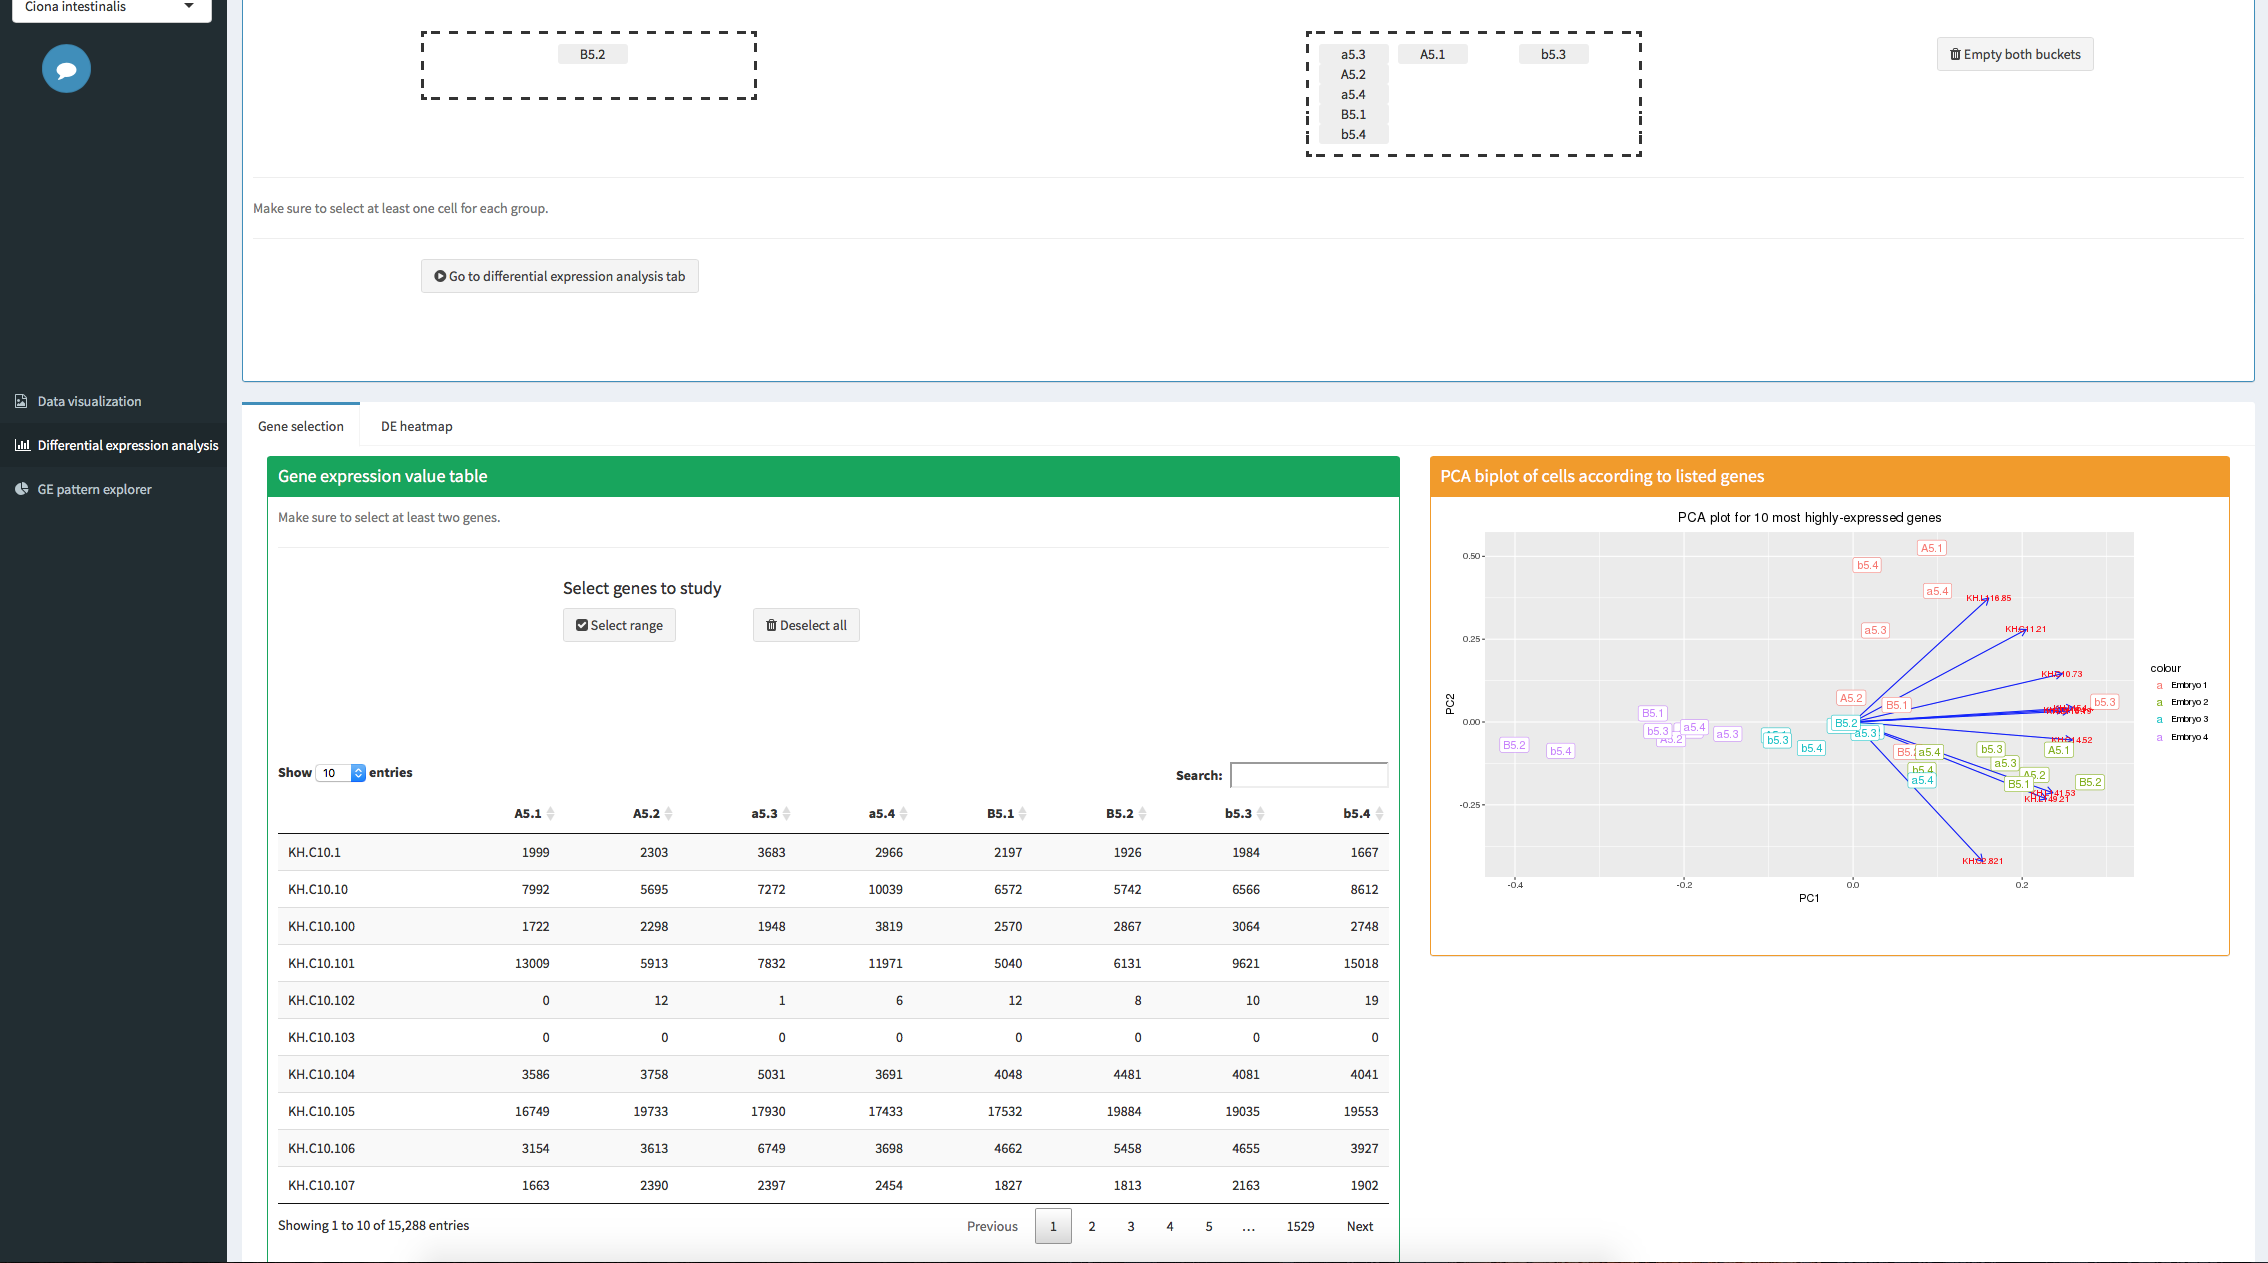
\includegraphics[scale=0.13]{Images/geneselection.png}
\caption{Screenshot of the application}
\end{figure}

\end{frame}

\subsection{Benchmark on clustering algorithms}

\begin{frame}
\tableofcontents[currentsubsection]
\end{frame}

\begin{frame}
\frametitle{Benchmark method (1/2)}

\begin{alertblock}{}
\begin{flushcenter}
Each algorithm has been iterated 100 times on each dataset,\\ with the best parameter values.
\end{flushcenter}
\end{alertblock}

\begin{itemize}
\item \textbf{Accuracy} measure:

\begin{block}{Adjusted Rand Index}
Compares a resulting clustering $\mathscr{C}$ to a reference labelling\\of points $\mathscr{R}$.
\begin{enumerate}
\item If ARI($\mathscr{C}, \mathscr{R}$) = 1, then $\mathscr{C}$ and $\mathscr{R}$ are similar.
\pause
\item If ARI($\mathscr{C}, \mathscr{R}$) = 0, then the algorithm is not better than the random strategy.
\pause
\item If ARI($\mathscr{C}, \mathscr{R}$) < 0, then the two clusterings totally differ.
\end{enumerate}
\end{block}

\end{itemize}

\end{frame}

\begin{frame}
\frametitle{Examples for the ARI measure (1/2)}

\begin{figure}
\subfigure\includegraphics[scale=0.25]{Images/ciona_ref.png}
\subfigure\includegraphics[scale=0.25]{Images/ciona_dbscan.png}
\caption{ARI $\approx$ 0.007 (\textbf{[Suyama et al., unp.]} dataset)}
\end{figure}

\end{frame}

\begin{frame}
\frametitle{Examples for the ARI measure (2/2)}

\begin{figure}
\subfigure\includegraphics[scale=0.25]{Images/ciona_ref.png}
\subfigure\includegraphics[scale=0.25]{Images/ciona_sincera.png}
\caption{ARI $\approx$ -0.12 (\textbf{[Suyama et al., unp.]} dataset)}
\end{figure}

\end{frame}

\begin{frame}
\frametitle{Benchmark method (2/2)}

\begin{alertblock}{}
\begin{flushcenter}
Each algorithm has been iterated 100 times on each dataset,\\ with the best parameter values.
\end{flushcenter}
\end{alertblock}

\bigskip

\begin{itemize}
\item \textbf{Time complexity}: depending on the number of cells and number of genes.

\bigskip

\item \textbf{Stability}: study of the ARI index variation across all 100 iterations.
\end{itemize}

\end{frame}

\begin{frame}
\frametitle{Benchmark results (1/3)}

\begin{center}
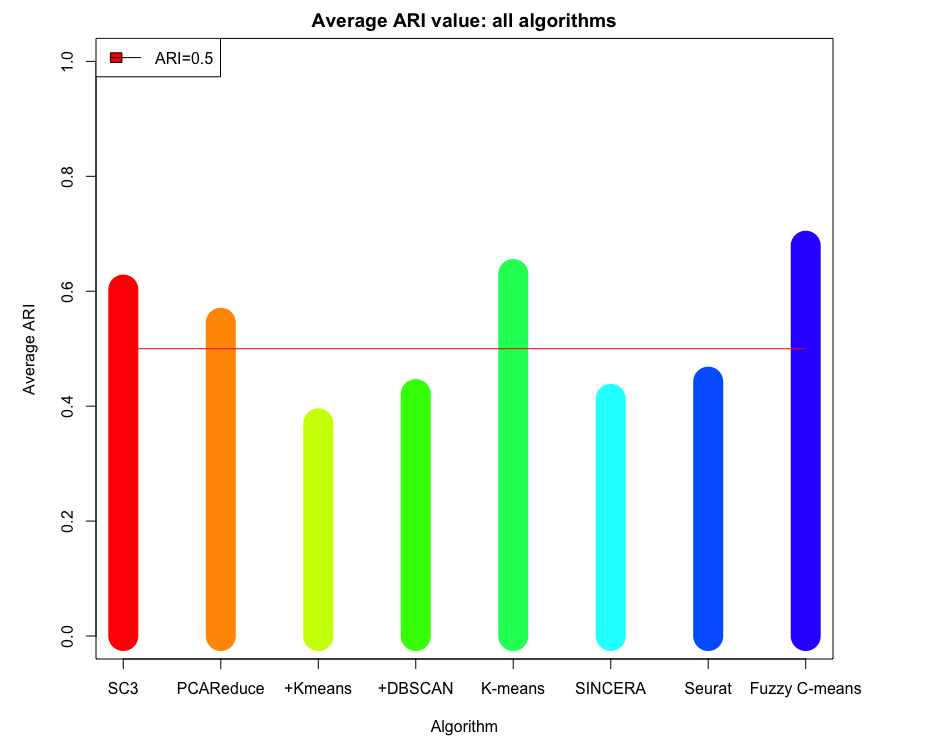
\includegraphics[scale=0.25]{Images/ariAverageAll.png}
\end{center}

\end{frame}

\begin{frame}
\frametitle{Benchmark results (2/3)}

\begin{center}
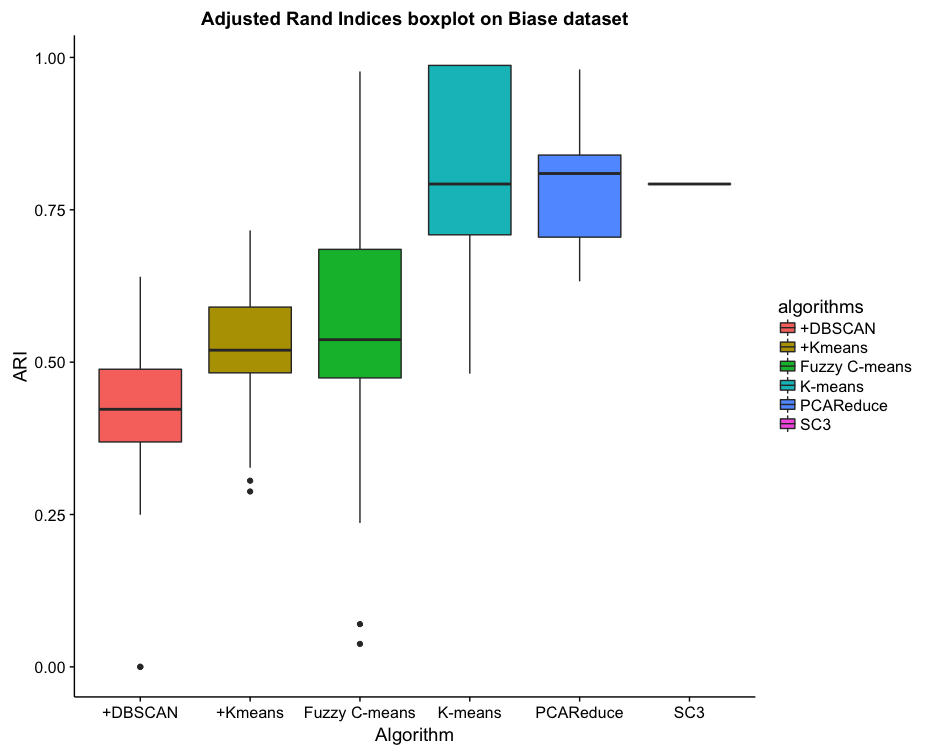
\includegraphics[scale=0.25]{Images/boxplotStability.png}
\end{center}

\end{frame}

\begin{frame}
\frametitle{Benchmark results (3/3)}

\begin{center}
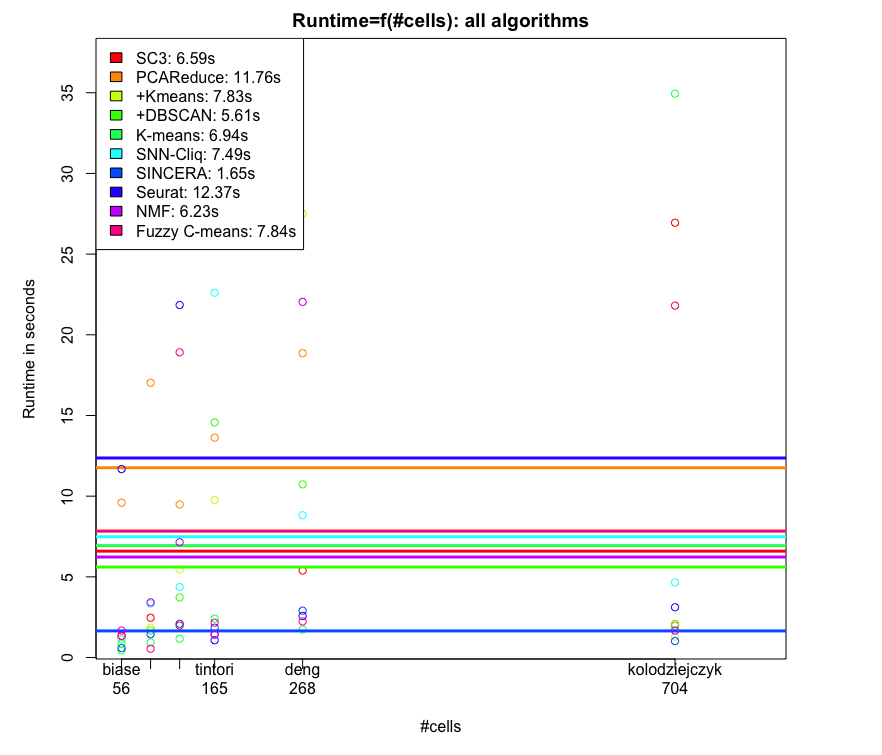
\includegraphics[scale=0.25]{Images/runtimeCellAll.png}
\end{center}

\end{frame}

\subsection{Gene expression model}

\begin{frame}
\tableofcontents[currentsubsection]
\end{frame}

\begin{frame}
\frametitle{Characteristics of \textit{\textbf{single-cell} RNA sequencing} data}

\begin{alertblock}{}
\begin{enumerate}[<+>]
\bigskip
\item Lots of \textbf{dropout} events \textbf{[Lun et al., 2016]}.
\item High cell-to-cell variability \textbf{[Martinez et al., 2017]}.
\item Log-"normal" model for gene expression \textbf{[Finak et al., 2015]}. 
\item Bimodal gene expression distribution \textbf{[McDavid et al., 2014]}, etc.
\bigskip
\end{enumerate}
\end{alertblock}

\end{frame}

\begin{frame}
\frametitle{A single cell gene expression model}

\begin{block}{Goal}
\begin{center}
Design a model to pseudo-randomly generate \textit{single cell gene expression data} from a small sample.
\end{center}
\end{block}

\pause

\begin{alertblock}{Core idea}
\begin{itemize}[<+>]
\item \textbf{Gene correlation}.
\item A \textbf{model for single gene expression} is known.
\item The \textbf{whole gene regulation system} is not known. 
\end{itemize}
\pause
\begin{flushcenter}
$\Rightarrow$ \textbf{Idea:} design separately \textbf{single gene expression}\\and \textbf{single cell gene expression}.
\end{flushcenter}
\end{alertblock}

\end{frame}

\begin{frame}
\frametitle{How to link gene-level expression and gene regulation?}

\begin{block}{Copula \textbf{(Sklar, 1959)}}
A multivariate joint CDF $\mathscr{C}$ which margins follow standard uniform distributions.
\pause
\bigskip

Let $U_1, U_2, U_3, ..., U_p$ $\thicksim \mathscr{U}_{0,1}$ r. v.: \\
\begin{center}
$\forall 0 \leq x_1 \leq 1, ..., 0 \leq x_p \leq 1,$\\$\mathscr{C} : x \rightarrow \mathbb{P}(U_1 \leq x_1 \land ... \land U_p \leq x_p)$
\end{center}
\end{block}

\end{frame}

\begin{frame}
\frametitle{Use of copula in modelling}

\begin{itemize}
\item $(X_i)_{i \in \{1, 2, ..., p\}}$ is a set of $\mathbb{R}$-valued r. v. with CDF $(\mathscr{F}_i)_{i \in \{1, 2, ..., p\}}$.
\item $\mathscr{F}$ is a joint CDF of $(X_i)_{i \in \{1, 2, ..., p\}}$, i.e.:\\
\begin{center}
$\forall x \in \mathbb{R}^p, \mathscr{F}(x_1, ..., x_p) = \mathbb{P}(X_1 \leq x_1, ..., X_p \leq x_p)$
\end{center}
\end{itemize}

\pause

\begin{alertblock}{Theorem \textbf{[Sklar, 1959]}} 
\begin{enumerate}[<+>]
\item Then there is a copula $\mathscr{C}$ such as: $\forall x \in \mathbb{R}$, $\mathscr{F}$($x_1, x_2, ..., x_p$) = $\mathscr{C}$($\mathscr{F}_1(x_1), \mathscr{F}_2(x_2), ..., \mathscr{F}_p(x_p)$).
\item Given a copula $\mathscr{D}$,\\$\mathscr{H}$ : $(\mathbb{R}^+)^p$ $\rightarrow$ $[0,1]$, $x$ $\rightarrow$ $\mathscr{D}$($\mathscr{F}_1(x_1), ..., \mathscr{F}_p(x_p))$ is a CDF.
\end{enumerate}
\end{alertblock}

\end{frame}

\begin{frame}
\frametitle{Which distributions should be chosen? (1/4)}

\begin{figure}
\centering
\includegraphics[scale=0.28]{Images/tintoriGene.png}
\caption{Dataset from \textbf{[Tintori et al., 2016]}}
\end{figure}

\end{frame}

\begin{frame}
\frametitle{Which distributions should be chosen? (2/4)}

\begin{figure}
\centering
\includegraphics[scale=0.28]{Images/tintoriCell.png}
\caption{Dataset from \textbf{[Tintori et al., 2016]}}
\end{figure}

\end{frame}

\begin{frame}
\frametitle{Which distributions should be chosen? (3/4)}

\begin{figure}
\centering
\includegraphics[scale=0.28]{Images/correlationAllGene.png}
\caption{Dataset from \textbf{[Tintori et al., 2016]} (all genes)}
\end{figure}

\end{frame}

\begin{frame}
\frametitle{Which distributions should be chosen? (4/4)}

\begin{figure}
\centering
\includegraphics[scale=0.28]{Images/correlationiGenes.png}
\caption{\textbf{[Tintori et al., 2016]} (informative genes: thres=0.75)}
\end{figure}

\end{frame}

\begin{frame}
\frametitle{Model for single-cell gene expression}

After \textbf{feature selection}\\and computation of the \textbf{two modes} for each cell:
\pause
\begin{alertblock}{For a given cell $j$ and $p$ genes (log-normalized values)} 

\begin{itemize}
\item $\mathscr{C}_j_{\mu_1_j, \mu_2_j, \alpha_j, \Sigma}$ is a bimodal Gaussian copula of means: $\mu_1_j$, $\mu_2_j$, covariance: $\Sigma$, rate: $\alpha_j$.
\pause
\item $\forall i \leq p, X_{i,j}$ is the r.v. associated with expression of gene $i$.
\item $X_j = (X_{1,j}, ..., X_{p, j})$ is the r.\textbf{v}. associated with expression in cell $j$.
\pause
\item For all $i \leq p$, $\mathscr{F}_{X_{i,j}}$ (CDF of $X_{i,j}$) is the known model for single gene $i$ expression.
\end{itemize}
\pause
\begin{flushcenter} 
\matchbb{P}($X_j \leq q$) = $\mathscr{C}_j_{\mu_1_j, \mu_2_j, \alpha_j, \Sigma}(\phi^{-1} \circ \mathscr{F}_{X_{1,j}}(q_1), ..., \phi^{-1} \circ \mathscr{F}_{X_{p,j}}(q_p))$\end{flushcenter}
\end{alertblock}
\end{frame}

\begin{frame}
\frametitle{Results (1/2): values from dataset \textbf{[Tintori et al.]}}

\begin{figure}
\centering
\includegraphics[scale=0.32]{Images/geABemb3.png}
\end{figure}

\end{frame}

\begin{frame}
\frametitle{Results (2/2): generation from the model}

\begin{figure}
\centering
\includegraphics[scale=0.32]{Images/copulaABemb3.png}
\end{figure}

\end{frame}

\section{Outlook}

\begin{frame}
\tableofcontents[currentsection]
\end{frame}

\begin{frame}
\frametitle{Conclusion}

\begin{block}{Contribution}
\bigskip
\begin{enumerate}[<+>]
\item An online application for data analysis.
\bigskip
\item A benchmark performed on clustering algorithms.
\bigskip
\item A model for \textit{single-cell} gene expression, that needs improvement.
\end{enumerate}
\bigskip
\end{block}

\end{frame}

\end{document}
